\documentclass{beamer}

\usepackage{xcolor}
\usepackage{amsmath}
\usepackage{amssymb}
\usepackage{graphicx}


\title{CAPP: Cost-Aware Pushdown Planner}
\author{Mason Hall, Abhinav Sapkota, Shiv}
\institute{University of Cincinnati}
\date{\today}

\definecolor{UCRed}{HTML}{E00122}
\definecolor{UCDarkRed}{HTML}{B8011C}
\definecolor{UCBlack}{HTML}{000000}
\definecolor{UCGray}{HTML}{F3F3F3}
\definecolor{UCWhite}{HTML}{FFFFFF}

\usetheme{Antibes}
\usecolortheme{default}

\setbeamercolor{normal text}{
    fg=UCBlack,
    bg=UCWhite
}
\setbeamercolor{structure}{fg=UCRed}

\setbeamercolor{frametitle}{
    fg=UCWhite,
    bg=UCRed
}

\setbeamercolor{title}{
    fg=UCWhite,
    bg=UCRed
}
\setbeamercolor{subtitle}{
    fg=UCBlack
}

\setbeamercolor{block title}{
    fg=UCWhite,
    bg=UCRed
}
\setbeamercolor{block body}{
    fg=UCBlack,
    bg=UCGray
}

\setbeamertemplate{itemize item}{
    \color{UCRed}\small$\blacksquare$
}

\graphicspath{{./images/}}

\begin{document}

\maketitle

\section{Introduction}
\begin{frame}
    \textbf{Topic:}
    \begin{itemize}
        \item Distributed Database Systems \pause
        \item Distributed Query Strategies
    \end{itemize}
\end{frame}

\begin{frame}{Papers}
Two papers from the same lab at the University of Wisconsin \pause
\newline
    \begin{itemize}
        \item \textbf{Disaggregation} \pause
        \item \textbf{PushdownDB}
    \end{itemize}
\end{frame}

\subsection{Papers}
\begin{frame}{Disaggregation}
    \begin{itemize}
        \item Describes the current state of distributed database architectures \pause
            \begin{itemize}
                \item Utilize popular clouds (AWS, GCP, etc.) \pause
                \item Split up components into specialized products (EC2
                for compute, S3 for storage) \pause
            \end{itemize}
        \item States that distributed query planning is an open problem
    \end{itemize}
\end{frame}

\begin{frame}{PushdownDB}
    \begin{itemize}
        \item Explores the AWS product \textit{S3 Select} \pause
        \begin{itemize}
            \item Storage product like S3 \pause
            \item Supports SQL filtering of data to be returned \pause
        \end{itemize}
        \item States that pushing filters into S3 is "always cost-effective" \pause
    \end{itemize}
\end{frame}

\begin{frame}{PushdownDB cont.}
\textbf{Results/Costs}
    \begin{figure}
        \centering
        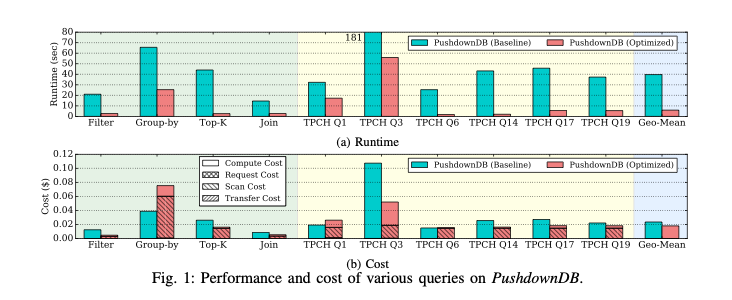
\includegraphics[scale=0.4]{PushdownDBResults}
    \end{figure}
    \begin{figure}
        \centering
        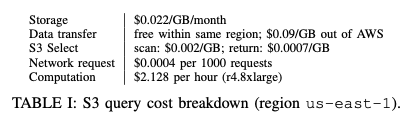
\includegraphics[scale=0.4]{PushdownDBCosts}
    \end{figure}
\end{frame}

\section{Solution}
\begin{frame}{Our Question}
    There are certainly some queries where paying to do the scan on S3 costs more. \pause
    \newline
    \newline
    \textbf{Example:} A predicate that would return 99\% of the data. \pause
    \begin{enumerate}
        \item Scan all the data to filter out results \pause
        \item Return basically all of it anyway \pause
        \item Pay select scan cost for no reason \pause
    \end{enumerate}
    \textbf{Q: When is the best time to push down vs. pull?}
\end{frame}

\begin{frame}{Query Planner}{What is it?}
    \begin{itemize}
        \item SQL is declarative; say what you want, not how to do it
        \item Planner's job: decide how to perform the given query
        \item
    \end{itemize}
\end{frame}

\section{Results}
\begin{frame}
\end{frame}

\section{Conclusion}
\begin{frame}
\end{frame}

\end{document}
